El control del brazo se implementa mediante una máquina de estados finitos que define cuatro posiciones operacionales discretas. Cada posición corresponde a una configuración angular específica de los servomotores, optimizada para una fase del ciclo de cosecha (Tabla \ref{tab:estados_brazo}).

\begin{table}[H]
\centering
\small
\begin{tabular}{|l|c|c|c|p{4.5cm}|}
\hline
\textbf{Posición} & \textbf{Servo 1 (codo)} & \textbf{Servo 2 (hombro)} & \textbf{Gripper} & \textbf{Función} \\
\hline
Movimiento & -90° & -45° & Cualquiera & Brazo plegado para desplazamientos XY \\
\hline
Recoger & -20° & 20° & Abierto & Aproximación para recolección \\
\hline
Transportar & -70° & 70° & Cerrado & Transporte seguro de planta \\
\hline
Depositar & -20° & -20° & Abierto & Liberación sobre contenedor \\
\hline
\end{tabular}
\caption{\textit{Posiciones operacionales del brazo robótico}}
\label{tab:estados_brazo}
\end{table}

\begin{figure}[H]
    \centering
    % Fila superior
    \begin{subfigure}[b]{0.35\textwidth}
        \centering
        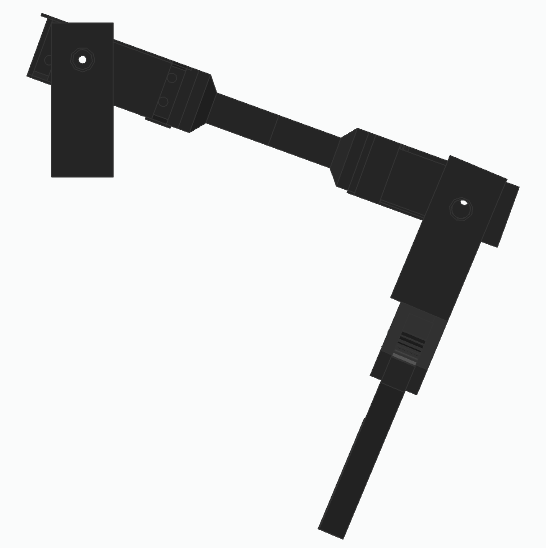
\includegraphics[width=\textwidth]{imagenes/brazo_movimiento.png}
        \caption{Posición Movimiento}
    \end{subfigure}
    \hfill
    \begin{subfigure}[b]{0.35\textwidth}
        \centering
        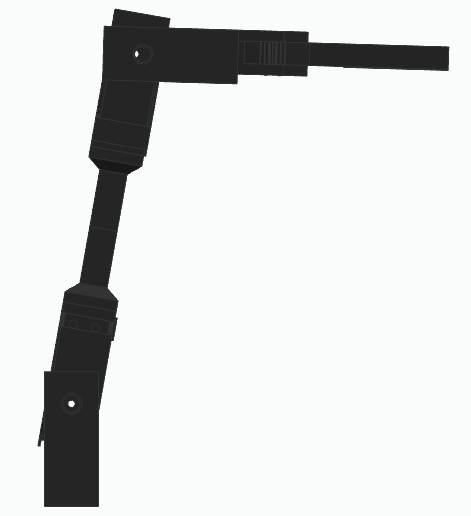
\includegraphics[width=\textwidth]{imagenes/brazo_transportar.png}
        \caption{Posición Transportar}
    \end{subfigure}

    % Espacio moderado entre filas
    \vspace{0.25cm}

    % Fila inferior
    \begin{subfigure}[b]{0.45\textwidth}
        \centering
        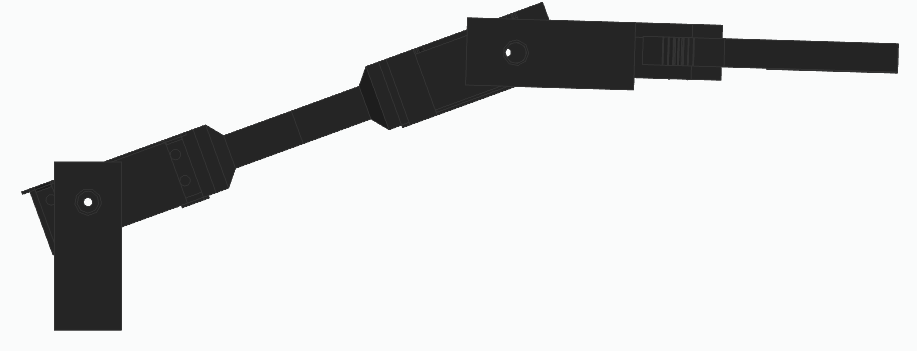
\includegraphics[width=\textwidth]{imagenes/brazo_recoger.png}
        \caption{Posición Recoger}
    \end{subfigure}
    \hfill
    \begin{subfigure}[b]{0.45\textwidth}
        \centering
        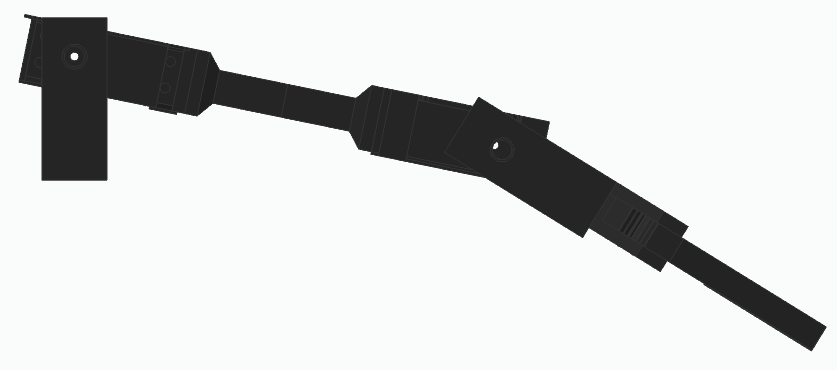
\includegraphics[width=\textwidth]{imagenes/brazo_depositar.png}
        \caption{Posición Depositar}
    \end{subfigure}

    \caption{\textit{Cuatro posiciones operacionales del brazo robótico}}
    \label{fig:posiciones_brazo}
\end{figure}


Las transiciones entre posiciones se ejecutan mediante interpolación lineal de ángulos. Dada una transición desde la posición A hacia la posición B, el sistema genera una trayectoria continua dividida en puntos intermedios muestreados cada 50ms durante un período $T$ de 1 a 3 segundos. Para cada servomotor $i$, el ángulo en el instante $t$ se calcula según:

\begin{equation}
\theta_i(t) = \theta_i^A + \frac{t}{T} \cdot (\theta_i^B - \theta_i^A)
\end{equation}

Esta interpolación garantiza movimientos suaves que minimizan vibraciones mecánicas y cargas sobre los actuadores. Las transiciones están reguladas por condiciones que verifican la validez de cada cambio de estado, evitando secuencias que comprometan la seguridad o integridad del sistema. 

Los movimientos del sistema cartesiano solo se permiten cuando el brazo se encuentra en posición de movimiento o transporte, garantizando que no ocurran colisiones durante desplazamientos. Mientras el brazo ejecuta una trayectoria de transición, se bloquean tanto comandos de movimiento XY como nuevas transiciones del brazo. Para algunos movimientos críticos, el robot debe estar en una posición XY determinada para evitar colisiones con el entorno.